



%##########################################################
\frontmatter
%##########################################################

\titlehead{\Large Technische Universit\"at Dresden\\
           Institut f\"ur Wirtschaft und Verkehr\\
           Lehrstuhl f\"ur \"Okonometrie und Statistik, insbes. im Verkehrswesen}
\subject{\Large Skript zur Vorlesung}
\title{{\Huge Verkehrs\"okonometrie}\\[5mm]
 {\LARGE Methoden und Modelle}}

\author{\LARGE Dr. Martin Treiber}

\date{\Large Wintersemester 2021/22}
\publishers{\small\copyright{} 2008-2022 Martin Treiber. 

%Dieses Skript darf nur zu Zwecken der Vorbereitung auf Vorlesung,
%\"Ubungen oder Klausur des Faches 
%``Grundlagen der Theoretischen Verkehrsplanung'' der TU Dresden vervielf\"altigt oder an
%Kommiliton(inn)en weitergegeben werden. Jede dar\"uber hinaus gehende
%Vervielf\"altigung oder Weitergabe des Skripts, oder von Teilen davon,
%bedarf der Zustimmung der Autoren, die in begr\"undeten F\"allen
% gern erteilt wird
%(email an \texttt{treiber\symbol{64}vwi.tu-dresden.de}). Auf die
%Quelle %vpl_skript passwortgesch!
%und das Copyright ist unbedingt
%hinzuweisen.
 
}
\maketitle

%####################

\tableofcontents

%##############

\mainmatter


%#########################################################
\chapter{\label{sec:Allg}Allgemeines}
%#########################################################


Das Wort \bfdef{\"Okonometrie} hat seinen Ursprung von der \"Okonomie
(Wirtschaft) und dem lateinischem Wort \textit{metiri}, welches
''messen'' bedeutet. Damit beinhaltet \"Okonometrie nicht nur \textit{quantitative}
wirtschaftliche Theorien und Konzepte, sondern vor allem deren
\bfdef{empirische} (also auf Messung, Beobachtung und Erfahrung beruhende)
\textit{\"Uberpr\"ufung}. 
Bei den durch Messung und Beobachtung gewonnen Daten handelt es sich
fast immer um \bfdef{statistische Daten}, also um eine
Beschreibung von \textit{Massenph\"anomenen}. Damit spielt neben der
quantitativen Formulierung wirtschaftlicher Theorien durch
\bfdef{mathematische Modelle} auch die Auswertung der
Daten durch \bfdef{statistische Modelle} eine Rolle. Das
Zusammenspiel der verschiedenen Elemente der \"Okonometrie wird in
folgendem Flussdiagramm deutlich.
 
\fig{\textwidth}{figsAllg/oekonometrieDef.eps}

In der Verkehrs\"okonometrie werden diese allgemeinen
Konzepte auf den
Verkehrssektor spezialisiert:

\maintext{Die \bfdef{Verkehrs\"okonometrie} umfasst die Gesamtheit
mathematischer Modelle und statistischer Verfahren, um auf einer
empirischen Grundlage den Verkehr und seine
 volkswirtschaftlichen Auswirkungen
quantitativ zu analysieren und zu prognostizieren.
}

%#########################################################
\section{\label{sec:oekonAblauf}Ablauf einer \"okonometrischen Untersuchung}
%#########################################################

Im Prinzip l\"auft eine \"okonometrische Untersuchung nach dem in
Abb.~\ref{fig:flussdiag-komplett} dargestellten Schema ab. Nach
Formulierung des Untersuchungsziels und dem Abgleich mit vergangenen
Untersuchungen kommt die wichtige Phase der Festlegung des
Erhebungsdesigns und des Modells. Diese beiden Komponenten m\"ussen
zusammenpassen. Will man beispielsweise ein Logit-Modell anwenden,
muss der Erhebungsfragebogen derart gestaltet sein, dass er eine
endliche Anzahl von Alternativen enth\"alt, welche (i)  \emph{alle}
m\"oglichen Antworten enthalten (Vollst\"andigkeit), (ii) jeweils nur
eine w\"ahlbar ist (Exklusivit\"at) und (iii) wesentlich voneinander
verschieden sind (sonst m\"usste man ein verallgemeinertes
Entscheidungsmodell anwenden). Ferner m\"ussen die Anzahl der
Variablen und ihre Skalierung (siehe 
unten) zur Modellspezifikation kompatibel sein. 

%#############################
\begin{figure}
\fig{0.6\textwidth}{figsErh/flussdiag-komplett.eps}
\caption{\label{fig:flussdiag-komplett}Allgemeiner
Ablauf einer \"okonometrischen 
Untersuchung.
}
\end{figure}
%#############################

Nach der dann folgenden Durchf\"uhrung der Datenerhebung
(Abschnitt~\ref{sec:erh}) werden die Modellparameter anhand der Daten
gesch\"atzt, also ihre wahrscheinlichsten Werte und ihr Streubereich
festgestellt. Die eigentliche Erkenntnis der \"okonometrischen
Untersuchung ergibt sich neben der deskriptiven Auswertung der
Erhebung vor allem anhand der Sch\"atzung der Modellparameter. Damit
lassen sich unter Anderem wichtige von unwichtigen Einflussfaktoren
trennen sowie Ma\3zahlen verkehrswirtschaftlicher Sachverhalte
gewinnen wie eine Bevorzugung bestimmter Verkehrsmittel (``bei
gleichem Zeit- und Kostenaufwand fahre ich lieber mit dem \"OV als dem
Auto'') oder implizite
Zeitwerte (``eine Stunde weniger Reisezeit ist mir 20 Euro wert''). 

%#########################################################
\section{\label{sec:oekonMod}Modelle und Variablen der Verkehrs\"okonometrie}
%#########################################################

Da die  \"Okonometrie wirtschaftliche Zusammenh\"ange quantitativ beschreibt,
besteht ihre Grundlage aus mathematischen Gleichungen. Generell kann
man \"okonometrische Modelle (und mathematische Modelle allgemein) als
eine mathematische Abbildung betrachten, die gewisse Eingabegr\"o\3en
auf Ausgabegr\"o\3en abbildet, wobei die Abbildung an den konkreten
Sachverhalt durch Modellparameter angepasst wird
(Abb.~\ref{fig:trichter}). Wir werden im Folgenden
Gleichungen folgender Struktur betrachten 
(vgl. Abb. \ref{fig:flussdiag}):

%###########################################
\begin{figure}
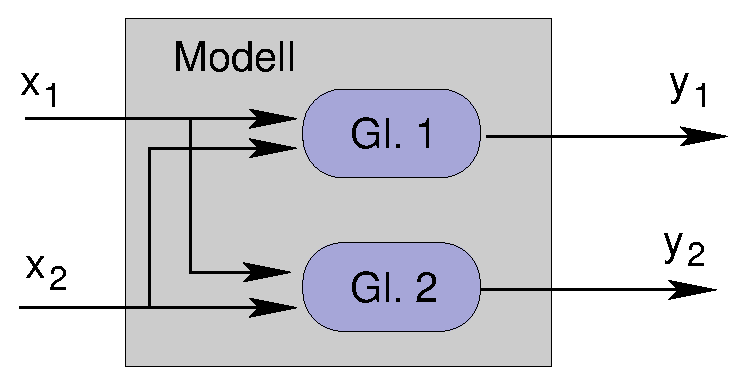
\includegraphics[width=0.49\textwidth]{figsAllg/flussdiag-Normal.eps}
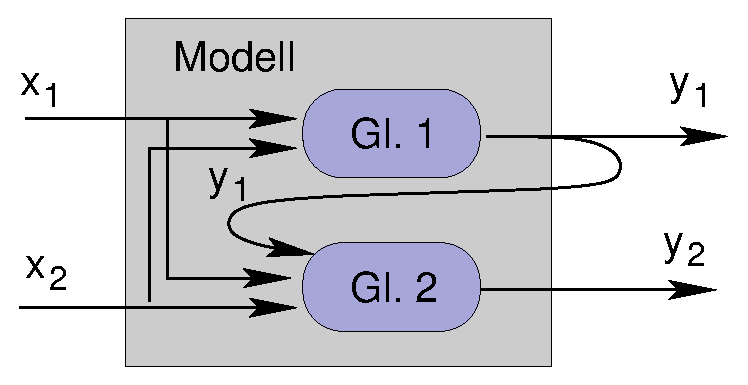
\includegraphics[width=0.49\textwidth]{figsAllg/flussdiag-Kopplung.eps}
\caption{\label{fig:flussdiag}Flussdiagramm der exogenen und
endogenen Variablen des allgemeinen \"okonometrischen Modells
\protect\refkl{oekonAllg}. Gezeigt ist der Fall f\"ur je zwei exogene und
endogene Variablen, $M=k=2$ ohne (links) und mit (rechts) Kopplung der
endogenen Variablen. Das Modell (eckige Box) besteht hier also
aus zwei Gleichungen, welche zwei Eingleichungsmodellen (links)
bzw. einem Mehrgleichungsmodell (rechts) entsprechen.
}
\end{figure}
%###########################################

%###########################################
\begin{figure}
\fig{0.35\textwidth}{figsAllg/ModellTrichter.eps}
\caption{\label{fig:trichter}''Flussdiagramm'' eines mathematischen
Modells in einer anfderen Perspektive: Oben kommen die exogenen
Variablen hinein, unten die endogenen heraus. Die Box stellt das
eigentliche Modell dar und die ``Stellschreauben'' die Modellparameter.
}
\end{figure}
%###########################################


\maineq{oekonAllg}{
Y_k=f_k(x_1, ..., x_m, ..,x_M, \beta_0, ..., \beta_j, ..., \beta_J)
+ \epsilon_k
= f_k(\vec{x}, \vec{\beta}) + \epsilon_k.
}

%################
\subsection{Endogene Variablen}
%################

Die $Y_k$ sind die \bfdef{erkl\"arten Variablen}.  Eine solche
Variable wird
bisweilen auch als \bfdef{Explanandum} (lat. ``zu erkl\"arende''
bzw. erkl\"arte Variable), als
\bfdef{endogene Variable} (Griechisch: von innen heraus, also aus dem
Modell kommend) oder gem\"a\3 allgemeinen mathematischen Sprachgebrauch als
\bfdef{abh\"angige Variable} bezeichnet. In der Systemtheorie
entsprechen die $Y_k$ dem \textit{Output} des jeweiligen Modells.
Da viele Modelle stochastischer Natur sind, also Zufallsgr\"o\3en
$\epsilon_k$ enthalten (vgl. Abschnitt~\ref{sec:genStoch}), 
sind die $Y_k$ im Allgemeinen Zufallsvariablen und
werden, der allgemeinen Konvention der Statistik entsprechend,
``gro\3'' geschrieben.

Je nach der Anzahl und Kopplung der endogenen Variablen werden
verschiedene Modellklassen unterschieden:
von
\bi
\item \bfdef{Eingleichungsmodelle}: Nur eine endogene Variable
$Y_1=Y$,
\item \bfdef{Mehrgleichungsmodelle}: Mehrere endogene  Variable $Y_k$, die
miteinander gekoppelt sind (vgl. Abb.~\ref{fig:flussdiag} rechts),
\item \bfdef{Mehreren Eingleichungsmodelle}: Mehrere ungekoppelte
endogene Variable wie im
Flussdiagramm~\ref{fig:flussdiag} links. Dies entspricht mehreren
separat zu l\"osenden Eingleichungsmodellen.
\ei

\textit{Beispiel Verkehrsmittelwahl}: Die $Y_k$ sind die absoluten
H\"aufigkeiten der gew\"ahlten Verkehrsmittel, z.B. $Y_1$=Zahl der
Kfz-Fahrten, $Y_2$=Zahl der \"OPNV-Fahrten und $Y_3$, $Y_4$ = Zahl der
Wege mit dem Rad bzw. zu Fu\3.

%################
\subsection{Exogene Variablen}
%################

Die Gr\"o\3en $x_m$, $m=1, \ldots, M$ sind die  \bfdef{erkl\"arenden
Variablen}, welche auch als  
\bfdef{Explanans} (lat. ``erkl\"arend''), \bfdef{exogene Variable}
 (Griechisch: von au\3en kommend) 
oder allgemein als
\bfdef{unabh\"angige Variable} bezeichnet werden.
 In der Systemtheorie
entsprechen die $x_m$ dem \textit{Input} in das jeweilige Modell.
In der Regel werden die $x_m$ als deterministisch betrachtet und
deshalb, der allgemeinen Konvention entsprechend, ``klein'' 
geschrieben.\footnote{In der Praxis werden sowohl die $x_m$ als auch
die $Y_k$ aus Erhebungen gewonnen, beide Variablenkategorien sind
damit  prinzipiell
stochastischer Natur. Man kann aber ohne
Einschr\"ankung der Allgemeinheit die Stochastizit\"at der
Input-Gr\"o\3en auf die Zufallsanteile $\epsilon_k$
verschieben, da die Modelle ja stochastische \textit{Funktionen}
darstellen, also die exogenen Variablen sowieso variabel sind. Dies
ist sogar geboten, da andernfalls die Stochastizit\"at
\"uberbestimmt ist. N\"aheres in Abschnitt~\ref{sec:genStoch}.}

Je anch Anzahl der exogenen Variablen definiert man
\bi
\item \bfdef{univariate Modelle}: $M=1$,
\item \bfdef{multivariate Modelle}\footnote{Streng genommen sind die
Termini Einfach- und Mehrfachregression in diesem Zusammenhang 
nicht korrekt, da sie eine spezielle Sch\"atzmethode (die Regression)
und nicht die Modelle als solches bezeichnen. Dies wird aber in der
Literatur h\"aufig ungenauerweise gleichgesetzt.}: $M>1$.
\ei

\textit{Beispiel Verkehrsmittelwahl}: Die $x_m$ sind die Reisezeiten
und andere, die Verkehrsmittelwahl beeinflussende Faktoren (Kosten,
Zuverl\"assigkeit etc)

%################
\subsection{Modellparameter}
%################

Die Gr\"o\3en $\beta_j$, $j=0, \ldots, J$ sind die \bfdef{Modellparameter}. Im
Gegensatz zu den exogenen und endogenen Variablen, welche sich bei
jedem System bzw. bei jeder Anwendung des
Modells \"andern, sollten die Modellparameter nach ihrer
\bfdef{Sch\"atzung} bzw. \bfdef{Modellkalibrierung} und einer
solcherma\3en bewirkten Anpassung des Modellverhaltens an die 
Wirklichkeit (vgl. Abschnitt
\ref{sec:kalib}) f\"ur alle Anwendungen
einen konstanten Wert besitzen.
\textit{Diese Eigenschaft ist ein entscheidendes Kriterium f\"ur die
Qualit\"at eines Modells und seiner Aussage- und Prognosekraft!}

\textit{Beispiel Verkehrsmittelwahl}: Modellparameter bestimmen die
relative Gewichtung einzelner Einflussfaktoren (z.B. f\"ur jedes
Verkehrsmittel den Wert der Zeit
in \euro{}/h) sowie eine a-Priori-Bevorzugung bestimmter Verkehrsmittel
gegen\"uber anderen  (in \euro{} oder Minuten) bei eigentlich gleichem Nutzwert.

%################
\subsection{\label{sec:genStoch}Zufallsanteile}
%################

Die $\epsilon_k$  beschreiben unbestimmte oder
\bfdef{nicht erkl\"arte Anteile} welche meist durch Zufallsvariablen
mit Erwartungswert $E(\epsilon_k)=0$ modelliert werden\footnote{Man
sagt,  dass ``Zufallselemente nichts anderes als das
Eingest\"andnis von Unwissen'' seien. Die Bedingung $E(\epsilon_k)=0$
ist keine Einschr\"ankung, da man einen eventuellen Erwartungswert auf
den deterministischen Teil verlagern kann.} 
Insbesondere gibt es folgende Gr\"unde f\"ur die Notwendigkeit eines
Zufallsanteils $\epsilon_k$:
\bi
\item Das Modell kann  nicht alle Einflussfaktoren
ber\"ucksichtigen. Wichtig ist aber, zumindest alle Faktoren mit
\emph{systematischen Einfluss} zu ber\"ucksichtigen, da das Modell
sonst \bfdef{fehlspezifiziert} ist und falsche Aussagen liefert
(vgl. Abschnitt~\ref{sec:spez}).
\item Die zur Modellkalibrierung verwendeten Messwerte sind
fehlerbehaftet. Dieser Anteil von $\epsilon$ gibt direkt die kumulierten
Messfehler wider.
\item Der Mensch ist keine Maschine. Der entsprechende Anteil von 
$\epsilon$ spiegelt die Abweichung des in Wirklichkeit oft
nichtrationalem Verhaltens vom Idealbild des \emph{Homo Oeconomicus}
wider.
\ei
Korrekt spezifizierte und eindeutig definierte 
Zufallsterme spielen eine wesentliche Rolle bei der
Parametersch\"atzung
(Abschnitt \ref{sec:kalib})

\textit{Beispiel Verkehrsmittelwahl}: $\epsilon_k$ entspricht dem
\emph{Zufallsnutzen}. Dieser sorgt daf\"ur, dass -- wie in der
Wirklichkeit -- mit geringerer Wahrscheinlichkeit auch ein
Verkehrsmittel mit nichtmaximalen deterministischen,
d.h. modellierten Nutzen gew\"ahlt wird.

%################
\subsection{Modellfunktionen}
%################

Die Funktionen $f_k(...)$ charakterisieren
schlie\3lich das eigentliche \"okonometrische
Modell. Wie bei den Parametern ist es f\"ur die G\"ute und
Prognosekraft eines Modells wichtig, dass es nach
seiner Entwicklung unver\"andert auf neue Instanzen des zu
beschreibenden Sachverhalts mit unterschiedlichen exogenen Variablen angewandt
werden kann.

\textit{Beispiel Verkehrsmittelwahl bei $N$ Entscheidungen insgesamt}: 
\bea
\label{allg-MNL-P}
P_k &=& \text{Prob}(\text{Altern $k$ gew\"ahlt}) 
  =  \frac{e^{V_k(\vec{x}, \vec{\beta})}}
  {\sum_{k'} e^{V_{k'}(\vec{x}, \vec{\beta})}}, \\
\label{allg-MNL}
Y_k & \sim & \text{Multinom}(N, \vec{P})\text{ - Verteilung.}
\eea
Dies ist ein verkettetes Modell (s. weiter unten) mit 2 Stufen:
\bi
\item 1. Stufe: Deterministisches Modell~\refkl{allg-MNL-P} f\"ur die
Auswahlwahrscheinlichkeiten
\item 2. Stufe: Stochastisches Modell~\refkl{allg-MNL}, welches
die Zufallsvariablen ``Zahl der Entscheidungen f\"ur Alternative $k$''
 mit Hilfe der Multinomialverteilung modelliert.
\ei
Die  Nutzenfunktionen $V_k(\vec{x}, \vec{\beta})$ enthalten die
Einflussfaktoren (exogenen Variablen) $\vec{x}$ (Reisezeit,
Kosten,...) und  die Modellparameter $\vec{\beta}=\{\beta_j\}$
(relative Gewichtungen und Bevorzugungen), w\"ahrend die zweite Stufe
keine weiteren exogenen Variablen oder Parameter enth\"alt.
N\"aheres dazu im Abschnitt
\ref{sec:choice}.

%##############
\subsection{Das Prinzip der Sparsamkeit}
%##############

Bei der Modellformulierung gilt das Sparsamkeitsprinzip
(\textit{principle of parsimony}), welches man, frei nach Einstein,
folgenderma\3en formulieren kann: 

\maintext{Das Modell sollte so einfach wie m\"oglich sein, aber nicht
einfacher.
Es sollte so wenig Parameter wie m\"oglich enthalten, aber nicht
weniger:

\textit{Mach' es so einfach wie m\"oglich, aber nicht einfacher} \quad\quad
(Albert Einstein)
}


%#########################################################
\section{\label{sec:oekonModgleichungen}Modellgleichungen}
%#########################################################

Die das \"okonometrische Modell beschreibenden mathematischen
Gleichungen 
 kann man nach zwei
Kriterien klassifizieren: Bez\"uglich der \textit{Inhaltlichen} bzw.
\textit{semantischen} Struktur und bez\"uglich der \textit{mathematischen} Struktur.

\subsection{Inhaltliche Struktur}

Hier unterscheidet man nach zwei Kategorien:
\bi
\item Das \bfdef{\"okonometrische Modell im engeren Sinn} 
wie Gl. \refkl{oekonAllg} beschreibt den \textit{abstrakten funktionalen
Zusammenhang}. Manchmal wird noch zwischen dem \emph{allgemeinen
Modell} (nicht spezifizierte Werte der Modellparameter) und dem
\emph{gesch\"atzten Modell} (nach der Parametersch\"atzung)
unterschieden.  Im einfachstm\"oglichen nichttrivialen Fall eines linearen
univariaten Eingleichungsmodells (eine exogene und eine endogene
Variable) lautet das allgemeine \"okonometrische Modell
\be
\label{allg-lin-einfach}
Y(x,\vecbeta)=\beta_0+\beta_1 x+\epsilon
\ee
und das gesch\"atzte Modell
\be
\hat{Y}(x)=\hat{\beta}_0+\hat{\beta}_1 x
\ee
Im \emph{allgemeinen Modell} haben die Parameter feste, aber noch nicht
bestimmte Werte und die Unsicherheit wird durch die Zufallsgr\"o\3e
$\epsilon$ ausgedr\"uckt. Im \emph{gesch\"atzten Modell}
gibt es keinen expliziten Zufallsterm mehr. Vielmehr sind die
Zufallseinfl\"usse auf die gesch\"atzten Parameterwerte
$\hat{\beta}_0$ und $\hat{\beta}_1$ \"ubergegangen, welche nun
\textit{ihrerseits} Zufallsvariablen darstellen.

Im Falle eines linearen multivariaten Eingleichungsmodells 
(mehrerer exogene und eine endogene Variable)
 lautet das allgemeine \"okonometrische Modell
\be
\label{allg-lin-mehrfach}
Y(x)=\beta_0+\sum_{m=1}^M\beta_m x_m+\epsilon
\ee

\item Die \bfdef{Systemgleichungen}, manchmal auch als
\bfdef{Messgleichungen} bezeichnet, beschreiben die
 \emph{Anwendung} des \"okonometrischen Modells auf
konkrete Systeme bzw. auf die von diesen Systemen gemessenen Werte der
exogenen und endogenen Variablen.  Im Gegensatz zum
abstrakten Modell h\"angen die Systemgleichungen vom
konkreten System ab. Die zum \"okonometrische
Modell~\refkl{allg-lin-einfach} geh\"origen Systemgleichungen lauten
\be
\label{allg-lin-einfach-system}
Y_i=\beta_0+\beta_1 x_i+\epsilon_i, \quad i=1, \ldots, n
\ee
und werden auf $n$ Datens\"atze $\{(x_i,y_i)\}$ angewandt. Die
Systemgleichungen zum
Mehrfachregressionsmodell~\refkl{allg-lin-mehrfach} lauten
\be
\label{allg-lin-mehrfach-system}
Y_i=\beta_0+\sum_{m=1}^M\beta_m x_{mi}+\epsilon_i
\ee
und werden auf $n$
Datens\"atze $\{(x_{1i},x_{2i}, ..., x_{Mi},y_i)\}$  angewandt. Mit Hilfe der
Systemgleichungen kann man die Modellparameter derart sch\"atzen, dass
eine Funktion $F(\{\epsilon_i\})$ der Modellierungsfehler
$\epsilon_i$, z.B. die Fehlerquadratsumme, minimal wird
(Kapitel~\ref{sec:kalib})
\ei



\noindent
\emph{Merke:} Wichtig ist es, bei einfach indizierten exogenen Variablen zu
unterscheiden, ob es sich um ein abstraktes Mehrfachregressionsmodell
der Art~\refkl{allg-lin-mehrfach} oder um Systemgleichungen eines
Einfachregressionsmodells der Art~\refkl{allg-lin-einfach-system} handelt.

\verstaendnisbox{Warum sollte es bei den Systemgleichungen 
immer mehr S\"atze von Messwerten geben als es der Zahl der Parameter
entspricht ($n>J+1$)? Was passiert, wenn $n=J+1$ oder gar $n<J+1$?
}




%#############################
\subsection{Mathematische Struktur}
%#############################

%#############################
\subsubsection{\label{sec:quasilin}Unterscheidung nach Linearit\"at}
%#############################

Die Unterscheidung ist in Hinblick auf die L\"osungsmethoden
wichtig. Man kann folgende Kategorien unterscheiden:
\bi
\item \bfdef{Lineare Modelle}: Hier h\"angen die endogenen Variablen
linear von den exogenen Variablen $\vec{x}$ und den Parametern
$\vec{\beta}$ ab: Bei Eingleichungsmodellen haben sie
also die
Form
\be
\label{linMultiAllg}
Y(x)=\beta_0+ \sum\limits_{m=1}^M \beta_m x_m  + \epsilon .
\ee
In vielen \"okonometrischen Lehrb\"uchern werden ausschlie\3lich
lineare Modelle behandelt, in der Verkehrs\"okonometrie sind jedoch
auch nichtlinieare Modelle wichtig.

\textit{Beispiel}: Einfaches Modell f\"ur die mittlere
Fahrleistung $Y$ pro Person in einer Region:
\be
\label{linExample}
Y=\beta_0+\beta_1 x_1+\beta_2 x_2+\beta_3 x_3
\ee
mit den erkl\"arenden Variablen
\bi
\item $x_1$: Mittleres Einkommen (Euro pro Jahr)
\item $x_2$: Treibstoffpreis (Euro/Liter)
\item $x_3$: Ausbau des Stra\3ennetzes (Kilometer pro Einwohner)
\ei
Als Aussagen lassen sich hier zum Beispiel Elastizit\"aten gewinnen
wie
\bdm
\epsilon_2=\frac{x_2}{Y}\abl{Y}{x_2}=\frac{\beta_2x_2}{Y}
\edm
Ein Wert $\epsilon_2=-0.2$ sagt z.B. aus, dass bei einer Erh\"ohung
der Treibstoffpreise um 10\% nur 2\% weniger Auto gefahren wird.

\item \bfdef{Reduzible nichtlineare Modelle}: Zwar h\"angt hier
die endogene 
Variable nichtlinear von sowohl den exogenen Variablen $\vec{x}$ als
auch den Parametern $\vec{\beta}$ ab, man kann die Modellgleichungen
jedoch  durch Transformation der
exogenen und/oder endogenen Variablen in eine lineare Form bringen. 

\emph{Beispiel:} Modell f\"ur das
\emph{unbeschr\"ankte Wachstum} eines \"okonomischen Prozesses
(z.B. die anf\"anglichen Verkaufszahlen eines neu eingef\"uhrten
Produkts). Mit der Zeit als exogenen Variablen lautet dieses

\be
\label{unlimitedGrowth}
y(t)=y_0e^{t/\tau+\epsilon}
\ee
Durch die Transformation $y=e^w$ und anschlie\3ende Logarithmierung
 wird dieses in ein lineares
Eingleichungsmodell transformiert:
\be
\label{unlimitedGrowthLog}
w(t)=\ln(y_0)+t/\tau+\epsilon=\beta_0+\beta_1 t+\epsilon
\ee
\verstaendnisbox{Warum funktioniert dies blo\3, wenn die
Zufallsanteile im urspr\"unglichen Modell \emph{multiplikativ} wirken?
}


%##################
\begin{figure}
\fig{0.6\textwidth}{figsAllg/limitedGrowth.eps}
\caption{\label{fig:limitedGrowth} Graph des
Modells~\refkl{limitedGrowth}.
}
\end{figure}
%##################


\item \bfdef{Irreduzible nichtlineare Modelle}: Hier h\"angt die endogene
Variable nichtlinear sowohl von den exogenen Variablen $\vec{x}$ als
auch von den Parametern ab und es ist keine Transformation auf eine
lineare Form m\"oglich. Dies ist zwingend immer dann der Fall,
wenn die endogenen Variablen \emph{diskreter Natur} sind (z.B. $Y=$ Zahl der
Wege, die mit dem Rad zur\"uckgelegt werden) oder wenn es sich gar um
\bfdef{qualitative} bzw. \bfdef{nominalskalierte Variablen} handelt,
z.B. $Y=$ gew\"ahlter Beruf mit den Auspr\"agungen Maurer, Schreiner,
Physiker etc. Aber auch im Bereich der stetigen Modelle gibt es
manchmal die Notwendigkeit von nichtlinearen Modellen, wie im
folgenden Beispiel.

\emph{Beispiel:} Modell f\"ur das
\emph{S\"attigungsverhalten} eines \"okonomischen
Prozesses (z.B. die Verkaufszahlen von Autos oder Mobiltelefonen seit
Erfindung der jeweiligen Produkte) beschreiben will. Das klassische
\bfdef{Modell beschr\"ankten Wachstums} mit der Zeit $x$ als exogenen
Variablen hat die Form (vgl. Abb.~\ref{fig:limitedGrowth})

\be
\label{limitedGrowth}
\hat{y}(x)=\frac{y_s}{1+\left(\frac{y_s}{y_0}-1\right)e^{-x/\tau}}
\ee


\verstaendnisbox{Diskutieren Sie die Bedeutung der Parameter $\tau$,
$y_0$ und $y_s$ im Modell~\refkl{limitedGrowth}. Kann man das Modell
auch in der Form 
$\hat{y}(x)=y_s/[1+e^{-(x-x_0)/\tau}]$ schreiben? Was ist dann die
Bedeutung des neuen Parameters $x_0$ und wie h\"angt er mit den
Parametern der Formulierung~\eqref{limitedGrowth} zusammen?
}

\item \bfdef{Quasilineare} bzw. \bfdef{parameterlineare Modelle}:
In dieser Modellklasse sind die Modellgleichungen 
linear bez\"uglich der Parameter $\vec{\beta}$,  aber
nichtlinear bez\"uglich der exogenen Variablen $\vec{x}$. Solche
Modelle kann man immer durch eine Transformation der exogenen
Variablen linearisieren,\footnote{Im Gegensatz zu den reduziblen
nichtlinearen Modellen gibt es hier auch keine Probleme mit den
Zufallsanteilen.} so dass sie \emph{v\"ollig \"aquivalent} zu den
linearen Modellen sind.
\maintext{Alle Methoden linearer Modelle sind identisch auch auf
die transformierten quasilinearen Modelle anwendbar. Im weiteren Verlauf
dieses Skriptes sind deshalb bei linearen Modellen immer auch
quasilineare Modelle mit eingeschlossen.}


\textit{Beispiel}: Einfaches Modell f\"ur die mittlere
PKW-Fahrleistung $Y$ eines PKW-Besitzers pro Jahr:
\be
\label{quasilinExample}
Y(\vec{x}, \vec{\beta})=\beta_0+\beta_1 x_1+\beta_2 x_2+\beta_3
x_1x_2+\epsilon 
\ee
mit den exogenen Variablen
\bi
\item $x_1$: Mittleres Einkommen (Euro pro Jahr)
\item $x_2$: Treibstoffpreis (Euro/Liter)
\ei
Mit den Transformationen 
\bdm
z_1=x_1, \quad z_2=x_2, \quad z_3=x_1x_2
\edm
wird dieses Modell in ein lineares Modell mit \emph{drei} exogenen
Variablen transformiert:
\be
\label{quasilinExample-ii}
Y(\vec{z}, \vec{\beta})=\beta_0+\beta_1 z_1+\beta_2 z_2+\beta_3 z_3
+\epsilon   
\ee
Die zugeh\"origen Anstiegsparameter bedeuten
\bi
\item $\beta_1$: Anstieg der Fahrleistung mit dem  Einkommen
(\"ublicherweise $\beta_1>0$)
\item $\beta_2$: Preissensitivit\"at der PKW-Nutzung 
(\"ublicherweise $\beta_2<0$)
\item $\beta_3$: Reduktion der Preissensitivit\"at mit dem Einkommen
(\"ublicherweise $\beta_3>0$)
\ei
\verstaendnisbox{Machen Sie sich die Vorzeichen der drei Parameter in
diesem Beispiel klar. Warum ist bei Ber\"ucksichtigung auch extrem
hoher Einkommen ein irreduzibel nichtlineares Modell notwendig? Zeigen
Sie dies anhand der dann nicht plausiblen Aussagen des
Modells~\eqref{quasilinExample-ii}.
}
\ei

%###########################################
\begin{figure}[t!]
\fig{0.8\textwidth}{figsAllg/flussdiag-Verkettung.eps}
\fig{0.8\textwidth}{figsAllg/flussdiag-Rueckkopplung.eps}
\caption{\label{fig:flussdiag-Kopplungen}Flussdiagramm der exogenen und
endogenen Variablen f\"ur verkette (oben) und
r\"uckgekoppelte (unten) Modell-Systeme. Das
``Innenleben'' der Modelle (also die je zwei Gleichungen,
vgl. Abb.~\ref{fig:flussdiag})  ist nicht
mehr gezeigt. Die Vektorpfeile symbolisieren den ganzen Satz
jeweiliger endogener und exogener Variablen.
}
\end{figure}
%###########################################


%###########################################
\begin{figure}[t!]
\fig{1.0\textwidth}{figsAllg/flussdiag-Zeitentwicklung.eps}
\caption{\label{fig:flussdiag-Zeitentwicklung}Flussdiagramm der
Verkettung im Falle dynamischer Modelle. Das Modell selbst ist in der
Regel in allen Schritten dasselbe, oft mit unver\"anderten Parametern
(\textit{autonomes} dynamisches Modell), manchmal mit von der Zeit
abh\"angigen (\textit{nichtautonomes} Modell).
}
\end{figure}
%###########################################

%#############################
\subsubsection{Unterscheidung nach weiteren mathematischen Kriterien}
%#############################

Weitere in der \"Okonometrie relevante Unterscheidungsmerkmale sind
\bi
\item Existenz eines Zufallsanteils: 
\bfdef{Deterministische} \textit{vs.} \bfdef{stochastische}
Modelle. 

\item Zahl der exogenen Variablen:
Eine bei univariaten und mehrere bei multivariaten Modellen.

\item Zahl der endogenen Variablen: Eine bei
Eingleichungsmodellen, mehrere bei Mehrgleichungsmodellen.

\item Skalierung der endogenen Variablen:
\bfdef{Entscheidungsmodelle} haben diskrete
bzw. qualitative/nominalskalierte endogene Variablen, w\"ahrend
\bfdef{kontinuierliche Modelle} stetige sowie verh\"altnisskalierte
 endogene Variable aufweisen. Diese beiden Kategorien bedingen
grunds\"atzlich verschiedene Herangehensweisen bei der Modellierung,
beispielsweise sind Entscheidungsmodelle immer nichtlinear.
 
Hingegen ist die Skalierung der exogenen Variablen nicht so
bedeutsam, da man qualitative bzw. nominalskalierte exogene Variable
durch kardinalskalierte \bfdef{Pseudovariablen} der Art 1=Maurer, 2=Schreiner,
3=Physiker etc ausdr\"ucken kann.

\item Existenz von Verkettung oder R\"uckkopplung (siehe
Abb.~\ref{fig:flussdiag-Kopplungen} und Abb.~\ref{fig:vierstufenmodell}):
\bi
\item Bei \bfdef{verketteten Modellen}
 sind die endogenen Variablen einer Modellstufe die exogenen der
n\"achsten. Wichtigstes Beispiel daf\"ur ist das Vier-Stufen-Schema der
klassischen Verkehrsplanung (Abb. \ref{fig:vierstufenmodell}).
\item Bei \bfdef{r\"uckgekoppelten Modellen} koppeln die endogenen
Variablen   
eines Modells einer sp\"ateren Verkettungsstufe auf die exogenen
Variablen eines Modells einer fr\"uheren Verkettungsstufe zur\"uck. Beim
Vier-Stufen-Modell der Abb.~\ref{fig:vierstufenmodell} k\"onnen als
Folge der Routenwahl einzelne Netzelemente \"uberlastet, also verstaut
 werden. Die damit verbundenen Resiezeitverl\"angerungen
 beeinflussen wiederum die Ziel- und
ggf. die Verkehrsmittelwahl.
\ei

\item Dynamische \textit{vs.} statische Modelle: \bfdef{dynamische
Modelle}, also Modelle mit expliziten dynamischen Zeitbezug, stellen
einen Sonderfall der Verkettung im Zeitbereich dar: Die
Entwicklung des aktuellen Zeitschrittes h\"angt von den Ergebnissen des
vergangenen Zeitschrittes bzw. der vergangenen Zeitschritte ab
(Abb.~\ref{fig:flussdiag-Zeitentwicklung}).
Im Rahmen der Vorlesung werden wir einen einfachen Typ dieser Modelle
kennen lernen, das \bfdef{dynamische Input-Output-Modell} (Abschnitt
\ref{sec:IOM}). 

\ei



%###########################################
\begin{figure}[t!]
\fig{1.0\textwidth}{figsAllg/vierstufenmodell.eps}
\caption{\label{fig:vierstufenmodell}Das klassische Vierstufenmodell
der Verkehrsplanung als Beispiel der Verkettung und R\"uckkopplung von
Modellen. Die endogenen Variablen der ersten Modellstufe 
``Aktivit\"atenwahl'', die im Verlauf eines Tages anfallenden
Verkehrsstr\"ome von und nach jedem
Bezirk (Quell- bzw. Zielsummen), spielen gleichzeitig   die Rolle von
exogenen Variablen  
bei der Modellierung der ``Zielwahl''. Die endogenen Variablen der
Zielwahl (Quelle-Ziel-Relationen bzw. 
Wege zwischen jeweils zwei Bezirken) sind wiederum die
exogenen Variablen der Verkehrsmittelwahl und in weiterer Folge der
Routenwahl. Das Ergebnis der Routenwahl f\"uhrt ggf. zu einer
\"Uberlastung einzelner Netzelemente und zu einer Erh\"ohung der
Reisezeit auf einigen Relationen. Diese sogenante ``Reisezeitmatrix''
bzw. ``Aufwandsmatrix'' ist nun wiederum eine weitere exogene Variable
der Zielwahl (``wenn der Weg von Bezirk $i$ nach $j$ immer verstopft ist, gehe
ich vielleicht doch woanders einkaufen''), so dass die Routenwahl auf
die Zielwahl r\"uckkoppelt.
}
\end{figure}
%###########################################


%##########################################
\section{\label{introBsp}Ein Anwendungsbeispiel: Verkehrsmittelwahl}
%##########################################

Zur Veranschaulichung der in diesem Kapitel beschriebenen Konzepte
soll das folgende Beispiel der Modellierung einer Verkehrsmittelwahl
dienen. 

%##################
\subsection{Modellstruktur}
%##################

Das Beispiel enth\"alt als Verkettung die 
wichtigsten beiden der in dieser Vorlesung
behandelten Modellklassen (Abb.~\ref{fig:Aufteilung}):
\bi
\item In der ersten Stufe gibt es als Teilmodelle vier stetige
Eingleichungsmodelle, welche aus den exogenen Variablen 
\bi
\item Zeitbedarf $X_{1k}$ des Verkehrsmittels $k$,
\item Kosten $X_{2k}$ des Verkehrsmittels $k$,
\item Komfort $X_{3k}$ des Verkehrsmittels $k$
\ei
den deterministischen Nutzen $V_k$
des jeweiligen Modus als endogene Variable ausgeben.

\item Das eigentliche \emph{Wahlmodell} enth\"alt als verkettete exogene
Variablen die deterministischen Nutzenfunktionen $V_k$ 
der vier Alternativen und liefert die prognostizierten
Entscheidungszahlen $\hat{Y}_k$ f\"ur jede Alternative. In seiner
Eigenschaft als diskretes Mehrgleichungsmodell ist das Wahlmodell 
 notwendigerweise nichtlinear.
\ei

%#############################
\begin{figure}
\fig{\textwidth}{figsAllg/beispiel-aufteilung.eps}
\caption{\label{fig:Aufteilung}Beispiel eines zweistufigen \"okonometrischen
Wahlmodells. Zun\"achst werden in vier
voneinander unabh\"angigen stetigen Eingleichungsmodellen
 die deterministischen Nutzenfunktionen $V_k$
der verschiedenen Verkehrsmittel $k$ modelliert. Diese wiederum
spielen die Rolle von exogenen Variablen im eigentlichen Wahlmodell.
Dieses diskrete Mehrgleichungsmodell liefert letztendlich als endogene Variablen 
die Zahlen $Y_k$ der Entscheidungen f\"ur
Verkehrsmittel $k$. 
}
\end{figure}
%#############################


%##################################
\subsection{Modellgleichungen und Parameter}
%##################################

Die vier Modelle f\"ur die Nutzenfunktionen werden als voneinander
unabh\"angige 
lineare (oder auch quasilineare) Eingleichungsmodelle  formuliert:

\be
\label{beisp-modell-nutzen}
U_k(\vec{x}_k, \vec{\beta}_k)
= \beta_{0k}+\sum_{m=1}^3 \beta_{mk}x_{mk}+\epsilon_k
\ee
Hierbei bedeuten:\footnote{Die Parametrisierung ist nicht
vollst\"andig, es fehlen z.B. die sozio\"okonomischen Variablen (siehe
Kapitel~\ref{sec:choice}). Als einf\"uhrendes Beispiel dient das
vereinfachte Modell aber
hier seinen Zweck.}
\bi
\item $\beta_{0k}$: Globaler Bonus des Verkehrsmodus $k$
gegen\"uber Modus 1 (damit ist offensichtlich $\beta_{01}=0$),
\item $\beta_{1k}$: Zeitbewertung bei Verkehrsmodus $k$
(beispielsweise kann man die Zeit zu Fu\3 unangenehmer empfinden als
die Zeit im Kfz, dann gilt $0 > \beta_{11}>\beta_{14}$),
\item $\beta_{2k}$: Geldbewertung bei Verkehrsmodus $k$,
\item $\beta_{3k}$: Bewertung des Komforts bei Verkehrsmodus $k$.
\ei


Von diesen Nutzenfunktionen wird der deterministische Anteil
$\hat{U}_k=V_k$ sowie die \emph{Standardabweichung} $\beta_0$ des
Zufallsnutzens an das eigentliche Wahlmodell weitergegeben. 
Bei insgesamt $N$ vorzunehmenden Entscheidungen hat das einfachste und
am weitesten verbreitete Wahlmodell, das 
Multinomial-Logit-Modell, die Modellgleichung
\be
\label{beisp-MNL}
Y_k(\vec{V},\beta_0)=N P_k(\vec{V},\beta_0) = N\frac{e^{\beta_0V_k}}
  {\sum_{k'} e^{\beta_0V_{k'}}}.
\ee

%##################################
\subsection{Systemgleichungen}
%##################################

Da die verketteten intermedi\"aren Variablen $V_k$ nicht messbar sind,
muss man die Verkettung der Teilmodelle~\refkl{beisp-modell-nutzen}
und~\refkl{beisp-MNL}   als Black-Box betrachten. Damit gelangt man zu
einem Modell der Form~\refkl{allg-MNL} mit messbaren exogenen
Variablen $x_{mk}$ und endogenen Variablen $Y_k$.

Um dieses Modell zu sch\"atzen, ben\"otigt man $n$ Messungen jeweils
aller exogenen und endogenen Variablen. Eine ``Messung'' ist hier der
technische Ausdruck einer Befragung einer Person: Von jeder Person $i$
m\"ussen also folgende Werte erfragt werden:\footnote{Die Werte der exogenen
Variablen haben einen Dreifachindex, da die Menge der exogenen
Variablen bereits doppelt indiziert ist.}

\bdm
\{ \underbrace{\hspace{5ex} x_{mki}\hspace{5ex} 
     }_{\parbox{15ex}{{\small Eigenschaften\\der Modi}}},
    \underbrace{\hspace{7ex} y_{ki}\hspace{7ex} 
     }_{\parbox{20ex}{{\small Zahl Entscheidungen\\f\"ur Alternative $k$}}}
\}
\edm
\vspace{1ex}

\noindent
Nach einer erfolgreichen Befragung hat der Interviewer eine Tabelle, welche
folgenderma\3en aussehen kann:
\vspace{1em}

%#############################
\hspace{-1em}
\begin{tabular}{|l||l|l|l|l|l||l|l|l|}
\hline
\myBox{14mm}{Gr\"o\3e}&
\myBox{12mm}{Zeit-\\bedarf\\Auto}&
\myBox{12mm}{Kosten\\Auto} &
\myBox{12mm}{Subj.\\Komfort\\Auto (1-6)} &
\myBox{12mm}{Kompl.\\Reisezeit\\ \"OPNV}  & 
\myBox{6mm}{\ldots}  & 
\myBox{11mm}{Wahl-\\entsch.\\Auto} &
\myBox{11mm}{Wahl-\\entsch. \"OPNV} &
\myBox{6mm}{\ldots}  
\\ \hline
\myBox{15mm}{Variable} &  
$x_{11i}$ & $x_{21i}$ & $x_{31i}$ & $x_{12i}$ & \ldots & $y_{1i}$ & $y_{2i}$& \ldots
\\ \hline
Person 1 &
  \unit[20]{min} & \unit[2.50]{\euro{}} & 3 & \unit[30]{min} & \ldots & 0 & 1& \ldots \\
Person 2 &
  \unit[11]{min} & \unit[2.00]{\euro{}} & 1  & \unit[20]{min} & \ldots & 1 & 0& \ldots \\
Person 3 &
  \unit[34]{min} & \unit[4.00]{\euro{}} & 1  & \unit[15]{min} &\ldots & 0 & 1& \ldots \\
$\vdots$ & $\vdots$ & $\vdots$ & $\vdots$ & 
$\vdots$ & $\vdots$ & $\vdots$ &  $\vdots$ & $\vdots$ \\
\hline
\end{tabular}
\vspace{1em}

\noindent
Anhand der Tabelle und der Zahl $N_i$ der Entscheidungen, welche
Person $i$ insgesamt trifft, werden die Systemgleichungen formuliert,
\be
\label{allg-MNL-system}
 \hat{Y}_{ki}=N_i \frac{e^{V_k(\vec{x}_i, \vec{\beta})}}
  {\sum_{k'} e^{V_{k'}(\vec{x}_i, \vec{\beta})}}, \quad i=1, \ldots, n.
\ee
Hierbei fasst der Vektor $\vec{x}_i=\{x_{11i}, \ldots, x_{34i}\}$ die
f\"ur Person $i$ relevanten exogenen Variablen zusammen. Anhand der
Systemgleichungen wird der (f\"ur alle Personen gleiche!) Parametervektor $\vec{\beta}$
durch Vergleich der modellierten endogenen Variablen $\hat{Y}_{ki}$
mit den gemessenen (erfragten) endogenen Variablen $Y_{ki}$
gesch\"atzt.




%##############################################
\subsubsection{Aggregierung}
%##############################################

Grunds\"atzlich sind Modelle der Verkehrsmittelwahl
\bfdef{mikroskopisch}, betrachten also jede Entscheidung einzeln. Damit
kann auch nur eine der endogenen Variablen $y_k$ f\"ur Alternative $k$
gleich~1 sein, w\"ahrend alle anderen $y_{k'}$, $k'\neq k$, gleich~0
sein m\"ussen. In drei F\"allen ist eine \emph{Aggregierung}, also eine
\bfdef{makroskopische Hernagehensweise}
m\"oglich, sinnvoll oder sogar notwendig:\footnote{Hier dient die
  Aggregierung  haupts\"achlich zu
  ``p\"adagogischen'' Zwecken, da sie die Darstellung vereinfacht. In
  Realit\"at wird man bei Vorliegen mikroskopischen Datenmaterials
  immer das mikroskopische Vorgehen w\"ahlen.}
\bi
\item \emph{personenbezogene Aggregierung:} 
Ein und dieselbe Person wird in vergleichbaren Situationen (gleiche
exogene Variable)
  mehrfach befragt. Geht es z.B. um die Verkehrsmittelwahl zur Arbeit
  und wurden die Entscheidungen
  den letzten zwei Wochen erhoben, kann man die 10~Entscheidungen zusammenfassen.
\item \emph{situationsbezogene Aggregierung:} 
W\"ahlt man die exogenen Variablen so, dass sie
f\"ur mehrere Personen \emph{und alle Alternativen} etwa gleiche Werte
besitzen, kann man diese Personen zu Gruppen bzw. Klassen zusammenfassen. In der
Praxis funktioniert dies meist nur, wenn man nur Variable w\"ahlt, welche
f\"ur alle Alternativen etwa gleich sind, also entweder
sozio\"okonomische Variable (Alter, Geschlecht, Autoverf\"ugbarkeit), externe Variable
(Wetter) oder spezielle generische Variable wie die Entfernung.
\item \emph{datenerzwungene Aggregierung:} Liegen Daten nur aggregiert
  vor, kann man nat\"urlich nur makroskopisch vorgehen.
\ei

%##############################################
\paragraph{Beispiel: mikroskopische Daten, welche eine Aggregierung
  zulassen (situationsbezogene Aggregierung)}

\begin{center}
 \begin{tabular}{|l||l|l|l|l||l|l|l|l|}
\hline
\myBox{12ex}{} & 
\myBox{6ex}{Entf. Fu\3} &
\myBox{6ex}{Entf. Rad} &
\myBox{6ex}{Entf. \"OPNV} &
\myBox{6ex}{Entf. MIV} &
\myBox{7ex}{Wahl-\\entsch. Fu\3} &
\myBox{7ex}{Wahl-\\entsch. Rad} &
\myBox{7ex}{Wahl-\\entsch. \"OPNV} &
\myBox{7ex}{Wahl-\\entsch. MIV}
\\ \hline
Variable &  
$x_{11}$ & $x_{12}$ & $x_{13}$ & $x_{14}$ & $y_1$ & $y_2$ & $y_3$ & $y_4$
\\ \hline
Person~1 &
  \unit[2]{km} & \unit[2]{km} & \unit[3]{km} & \unit[3]{km} & 0 & 1 & 0 & 0\\
Person~2 &
  \unit[4]{km} & \unit[4]{km} & \unit[4.5]{km} & $\infty$ & 0 & 0 & 1 & 0\\
Person~3 &
  \unit[3]{km} & \unit[3]{km} & $\infty$  & \unit[3.5]{km} & 0 & 0 & 0 & 1\\
$\vdots$ & $\vdots$ & $\vdots$ & $\vdots$ & 
$\vdots$ & $\vdots$ & $\vdots$ & $\vdots$ &  $\vdots$ \\
\hline
\end{tabular}
\end{center}

%##############################################
\paragraph{Aggregierung dieser Daten in Entfernungsklassen}
 
\begin{center}
 \begin{tabular}{|r||r|r|r|r||r|}
\hline
Entfernungsklasse &
\myBox{7ex}{Wahl-\\entsch. Fu\3} &
\myBox{7ex}{Wahl-\\entsch. Rad} &
\myBox{7ex}{Wahl-\\entsch. \"OPNV} &
\myBox{7ex}{Wahl-\\entsch. MIV} &
\myBox{7ex}{Pers.\\in Klasse}
\\ \hline
$x_{1}$ = Klassenmitte & $y_1$ & $y_2$ & $y_3$ & $y_4$ & $n_i$
\\ \hline
\unit[0-1]{km}   & 5 & 1 & 0 & 0 & 6\\
\unit[1-2]{km}   & 2 & 0 & 5 & 0 & 7\\
\unit[2-3]{km}   & 0 & 2 &11 & 0 &13\\
\unit[3-5]{km}   & 0 & 0 & 7 & 1 & 8\\
\unit[5-10]{km}  & 0 & 0 & 5 & 0 & 5\\
\unit[10-20]{km} & 0 & 0 & 1 & 1 & 2\\
\unit[$>20$]{km} & 0 & 0 & 3 & 0 & 3\\
\hline
$\sum$            & 7 & 3 &32 & 2 & 44\\
\hline
\end{tabular}

\end{center}

\newpage


%#########################################################
\section{\label{symbolsAllg}Verwendete Symbole}
%##########################################################

\begin{tabular}{ll}
\varDef{$Y$}{ Abh\"angige bzw. erkl\"arte bzw. endogene Variable. Bei
Mehrgleichungsmodellen bekommen diese den Index $k$.}
\varDef{$x_m$,\\$m=1, \ldots, M$}{Unabh\"angige bzw. erkl\"arende
bzw. exogene Variablen}
\varDef{$\vec{x}$}{Gesamtheit der exogenen Variablen, als Spaltenvektor
geschrieben}
\varDef{$y_i$, $x_{mi}$,\\$i=1, \ldots, n$}{Wert der abh\"angigen
bzw. der $m$-ten unabh\"angigen
Variablen bei der $i$-ten Messung bzw. dem $i$-ten Element der Stichprobe.}


\varDef{$\beta_0$}{Achsenabschnitt (engl. \textit{intercept})}
\varDef{$\beta_j$,\\$j=1, \ldots, J$}{Lineare Anstiegsparameter}
\varDef{$\vec{\beta}$}{Gesamtheit der Modellparameter, als Spaltenvektor
geschrieben}
\varDef{$\hat{\beta}_j$, $\hat{Y}$}{Das ``Dach'' ist ein Symbol f\"ur
gesch\"atzte Gr\"o\3en, also gesch\"atzte Parameterwerte, exogene Variable des
gesch\'atzten Modells, etc.}

\varDef{$\epsilon$}{Ein additiver i.i.d. Zufallsterm mit Erwartungswert 0 und der
Varianz $\sigma^2$}

\varDef{$z_m$, $w$}{Transformierte exogene und endogene Variablen (mit
dem Ziel, ein lineares Modell in den transformierten Variablen zu erhalten)}
\varDef{$V_k$}{Deterministische Nutzenfunktion der Alternative $k$ bei
Wahlmodellen}
\varDef{$U_k$}{Gesamtnutzen $V_k+\epsilon_k$ der Alternative $k$ bei
Wahlmodellen}

\varDef{$n$}{Zahl der Stichprobenelemente bzw. Messungen bzw. befragte
Personen (Laufindex $i=1, \ldots, n$)}
\varDef{$N$}{Zahl der Entscheidungen bei Wahlmodellen, $N=\sum_k Y_k$}
\varDef{$N_i$}{Zahl der Entscheidungen von Person $i$ bei
 Wahlmodellen, $N_i=\sum_k y_{ki}$}
\end{tabular}

